%% Direttive TeXworks:
% !TeX root = ./presentazione.tex
% !TEX encoding = UTF-8 Unicode
% !TEX program = arara
% !TEX TS-program = arara
% !TeX spellcheck = it-IT

% arara: pdflatex: { synctex: yes, action: batchmode, options: "-halt-on-error -file-line-error-style" }
% arara: biber
% arara: pdflatex: { synctex: yes, action: batchmode, options: "-halt-on-error -file-line-error-style" }
% arara: pdflatex: { synctex: yes, action: nonstopmode, options: "-halt-on-error -file-line-error-style" }

\documentclass[%
    % handout,      % serve per generare la versione stampabile
    % italian
]{beamer}

%% ORDINE IMPORTANTE INIZIO %%%%%%%%%%%%
\usepackage[T1]{fontenc}        % serve per impostare la codifica di output del font
\usepackage{textcomp}           % serve per fornire supporto ai Text Companion fonts
\usepackage[utf8]{inputenc}     % serve per impostare la codifica di input del font
\usepackage[
    english,        % utilizza l'inglese come lingua secondaria
    italian         % utlizza l'italiano come lingua primaria
]{%
    babel,                      % serve per scrivere Indice, Capitolo, etc in Italiano
    varioref                    % introduce il comando \vref da usarsi nello stesso modo del comune \ref per i riferimenti
}
\usepackage{lmodern}            % carica una variante Latin Modern prodotto dal GUST
%% ORDINE IMPORTANTE FINE %%%%%%%%%%%%%%
\usepackage{xcolor}             % serve per la gestione dei colori nel testo
\usepackage{graphicx}           % serve per includere immagini e grafici

%% Configurazione listings orribile, ma funziona %%%%%%%%%%%%%%%%%%%%
\usepackage{listings}           % serve ad inserire blocchi di codice
% \lstdefinelanguage{yaml}{
%     basicstyle=\scriptsize\sffamily\color{black},
%     string=[s]{"}{"},
%     stringstyle=\color{blue},
%     comment=[l]{:},
%     commentstyle=\color{blue},
%     frame=single,
%     numbers=left,
%     numbersep=5pt,
%     numberstyle=\tiny\color{gray},
%     showspaces=false,
%     showstringspaces=false,
%     tabsize=1
% }
\lstdefinelanguage{json}{
    basicstyle=\scriptsize\sffamily\color{black},
    string=[s]{"}{"},
    stringstyle=\color{black},
    comment=[l]{:},
    commentstyle=\color{blue},
    frame=single,
    numbers=left,
    numbersep=5pt,
    numberstyle=\tiny\color{gray},
    showspaces=false,
    showstringspaces=false,
    tabsize=1
}

\usepackage{subfigure}          % serve a creare sottofigure
\usepackage[%
    strict,             % rende tutti gli warning degli errori
    autostyle,          % imposta lo stile in base al linguaggio specificato in babel
    english=american,   % imposta lo stile per l'inglese
    italian=guillemets  % imposta lo stile per l'italiano
]{csquotes}                     % serve a impostare lo stile delle virgolette

\usepackage{silence}    % silenzia warning
\usepackage[%
    maxcitenames=2,     % massimo numero di nomi nelle citazioni
    mincitenames=2,     % minimo numero di nomi nelle citazioni
    maxbibnames=99,     % massimo numero di nomi nella blibliografia
    minbibnames=99,     % minimo numero di nomi nella blibliografia
    style=numeric,
    giveninits=true,
    backend=biber       % specifica il backend per la bibliografia
]{biblatex}                     % si interfaccia con bibtex e biber per la bibliografia
\addbibresource{biblio.bib}
%% Poiché il warning inutile di BibLaTeX non può essere rimosso, lo silenzio
%% https://tex.stackexchange.com/a/202994
\WarningFilter{biblatex}{Patching footnotes failed}
\setbeamertemplate{bibliography item}[text]

% \usepackage[%
%     %notbib,          % rimuove la bibliografia dall'indice
%     notindex,         % rimuove l'indice dall'indice
%     nottoc,           % rimuove la Table of Contents dall'indice
%     notlot,           % rimuove la lista delle tabelle dall'indice
%     notlof,           % rimuove la lista delle figure dall'indice
%     %chapter,         % "Use chapter-level headings, if possible"
%     %section,         % "Use section-level headings, if possible"
%     %numbib           % numera il capitolo della bibliografia
%     %numindex         % numera il capitolo dell'indice
% ]{tocbibind}                  % aggiunge cose all'indice

% \usetheme{CambridgeUS}        % TODO decidi quale usare
\usetheme{Boadilla}             % serve per scegliere il layout generale dei frame
\usecolortheme{beaver}          % Per il colore va comunque bene questo

\usepackage{pgf}
% \usepackage{pgfpages}         % serve per mettere più slide in una pagina
% \pgfpagesuselayout{4 on 1}[a4paper, border shrink=5mm, landscape]

% \usepackage[htt]{hyphenat}      % Enable hyphenation of TT text
\hyphenation{                   % Permette di sillabare bene le parole
    JavaFX
    Swing
    Micro-systems
    Script
    script
    Pack-age
    pack-age
    Manage-ment
    manage-ment
    Com-munity
    com-munity
}

\setcounter{secnumdepth}{2}     % Numera fino alla sottosezione nel corpo del testo
\setcounter{tocdepth}{3}        % Numera fino alla sotto-sottosezione nell'indice

\graphicspath{{img/}}

%% Definisco un nuovo comando per enfatizzare il testo in inglese %%%%%%%%%%%
\newcommand{\engEmph}[1] {\emph{\foreignlanguage{english}#1}}

%% ORDINE IMPORTANTE INIZIO %%%%%%%%%%%%
% hyperref va caricato il più tardi possibile
\usepackage{hyperxmp}           % Simile ad hyperref
\usepackage{hyperref}           % Gestisce tutte le cose ipertestuali del pdf
\hypersetup{%
    pdfpagemode={UseOutlines},
    hidelinks,          % nasconde i collegamenti (non vengono quadrettati)
    hypertexnames=false,
    linktoc=all,        % inserisce i link nell'indice
    bookmarks=true,
    bookmarksopen,
    bookmarksopenlevel=3,
    plainpages=false,
    breaklinks,
    pdfstartview={FitH},
    pdfauthor={Niccolò Maltoni},
    pdfcopyright={Copyright (C) 2017, Niccolò Maltoni},
    pdftitle={Progettazione object-oriented di un'interfaccia grafica JavaFX per il simulatore Alchemist},
    pdfcontactcountry={Italy},
    pdfcontactemail={niccolo.maltoni@studio.unibo.it},
    pdflang={it},
    pdfsubject={Lo scopo di questa tesi è la progettazione e la successiva implementazione di un'interfaccia grafica 2D per il simulatore Alchemist. La nuova interfaccia permette di interagire con la simulazione a tempo di esecuzione e di vedere chiaramente rappresentate informazioni su di essa. In particolare, è supportata una struttura modulare di effetti che rende facilmente osservabili determinate entità del sistema ed eventuali loro proprietà: rispetto alla classe di effetti dell'interfaccia classica, la nuova tipologia di effetti non è più una funzione dal singolo nodo alla rappresentazione grafica, bensì fa riferimento all'intero ambiente, permettendo di costruire rendering complessi facilmente esportabili tramite file JSON. Si è scelto di mantenere un'interfaccia il più possibile user-friendly, mantenendo un design più simile ai simulatori a scopo videoludico per favorire l'utilizzo da parte di utenti inesperti. Lo stile estetico al quale si è deciso di allinearsi è il Material Design di Google e la libreria grafica utilizzata per l'implementazione è stata JavaFX.},
    pdfkeywords={Progettazione object-oriented, Simulazione, Java, JavaFX, Interfaccia grafica},
    pdfa
}
% cleveref va anche dopo hyperref
\usepackage[%
    english,italian,    % definizione delle lingue da usare
    nameinlink          % inserisce i link nei riferimenti
]{cleveref}                     % permette di usare riferimenti migliori dei \ref e dei varioref
%% ORDINE IMPORTANTE FINE %%%%%%%%%%%%%%

\title[Nuova GUI Alchemist in JavaFX]{%
    Progettazione object-oriented di un'interfaccia grafica %
    JavaFX per il simulatore Alchemist
}
\subtitle{Tesi in Programmazione ad Oggetti}
\author[Niccolò~Maltoni]{Niccolò~Maltoni\\0000719734}
% \author[%
%     Niccolò~Maltoni \hspace{0.1\textwidth} \insertframenumber\,/\,\inserttotalframenumber%
% ]{%
%     Niccolò~Maltoni%
%     \\ \vspace{10pt} \small{Realtore: Prof.~Mirko~Viroli \\Correlatore: Prof.~Danilo~Pianini}%
% }
\date{%
    % TODO
}
\institute[%
    % Unibo
]{%
    Alma Mater Studiorum - Università di Bologna\\%
    Campus di Cesena%
}

% Permette di inserire l'outline prima di ogni sezione
\AtBeginSection[]{%
    \begin{frame}<beamer>
        \frametitle{Outline}
        \tableofcontents[currentsection]
    \end{frame}
}

\begin{document}
    \begin{frame}
        \titlepage
    \end{frame}

    \section{Introduzione}\label{sec:intro}
    \begin{frame}
        \frametitle{\insertsection}

        Lo scopo di questa tesi è la progettazione e la successiva implementazione di un'interfaccia grafica 2D per il simulatore \emph{Alchemist}~\cite{alchemist2013}.

        \medskip % non soono sicuro sia la soluzione più corretta, am funziona
        \pause

        La nuova interfaccia permette di interagire con la simulazione a tempo di esecuzione e di vedere chiaramente rappresentate informazioni su di essa.
    \end{frame}

    \begin{frame}
        \frametitle{\insertsection}

        In particolare, è supportata una \emph{struttura modulare di effetti} che rende facilmente osservabili determinate entità del sistema ed eventuali loro proprietà:

        \begin{itemize}[<+(1)->]
            \item
                l'effetto non fa più riferimento al singolo nodo, bensì costituisce una funzione dall'intero ambiente alla rappresentazione grafica.
            \item
                gli \engEmph{stack} di effetti realizzati possono essere serializzati su file di testo in formato JSON.
        \end{itemize}
    \end{frame}

    \begin{frame}
        \frametitle{\insertsection}

        Si è scelto di mantenere un'interfaccia il più possibile \engEmph{user-friendly}, mantenendo un design più simile ai simulatori a scopo videoludico per favorire l'utilizzo da parte di utenti inesperti.

        \medskip
        \pause

        Lo stile estetico al quale si è deciso di allinearsi è il \emph{Material Design} di Google\only<2->{\footnote{\url{https://material.io}}} e la libreria grafica utilizzata per l'implementazione è stata \emph{JavaFX}.
    \end{frame}

    \section{Alchemist}\label{sec:alchemist}

    \subsection{Introduzione ad Alchemist}\label{subsec:alchIntro}
    \begin{frame}
        \frametitle{\insertsection}
        \framesubtitle{\insertsubsection}

        Alchemist\only<1->{\footnote{\url{http://alchemistsimulator.github.io}}}~\cite{alchemist2013} è un meta-simulatore estendibile completamente open-source che esegue su Java Virtual Machine (JVM), nato all’interno dell’Università di Bologna e reperibile su GitHub\only<1->{\footnote{\url{https://github.com/AlchemistSimulator/Alchemist}}}.

        \medskip
        \pause

        L'idea dietro al progetto è quello di riuscire ad avere un framework di simulazione il più possibile generico, in grado di simulare sistemi di tipologia e complessità diverse, mantenendo le prestazioni dei simulatori non generici (come ad esempio quelli impiegati in ambito chimico~\cite{gillespie1976}).
    \end{frame}

    \subsection{Il modello di Alchemist}\label{subsec:alchModel}
    \begin{frame}
        \frametitle{\insertsection}
        \framesubtitle{\insertsubsection}

        \centering
        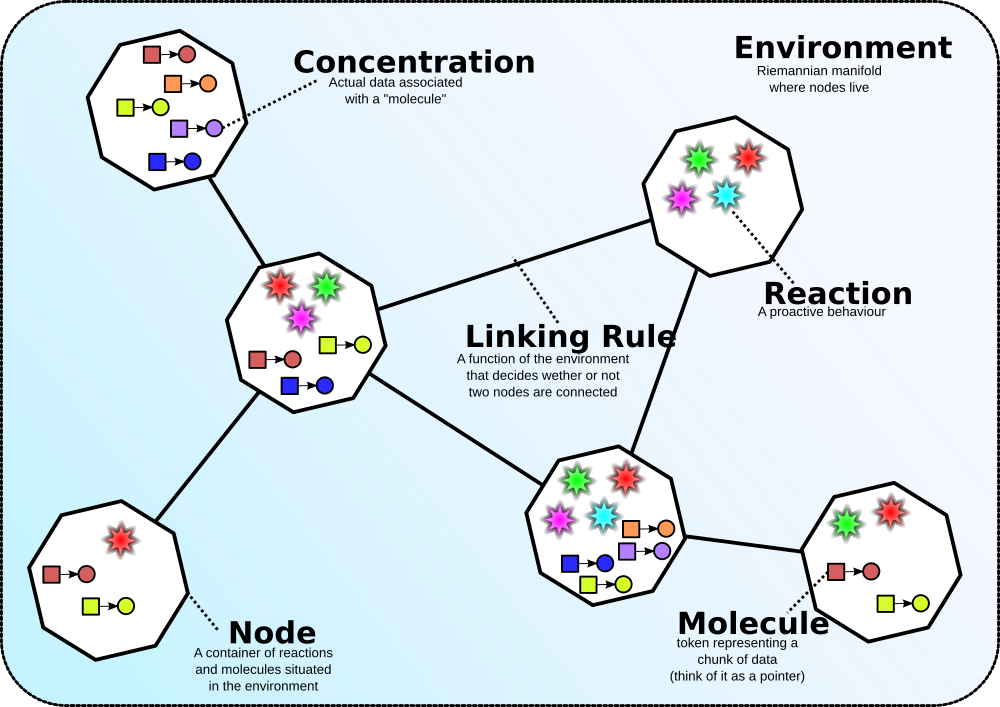
\includegraphics[scale=.34]{fig/alchemist_model}
    \end{frame}

    \begin{frame}
        \frametitle{\insertsection}
        \framesubtitle{\insertsubsection}

        \begin{description}[<+->]
            \item[Molecola]\label{itm:mol}
                Una \emph{Molecola} rappresenta il nome dato ad un particolare dato all'interno di un \emph{Nodo}, del quale ne astrae parte dello stato.

            \item[Concentrazione]\label{itm:conc}
                La \emph{Concentrazione} di una \emph{Molecola} è il valore associato alla proprietà rappresentata dalla \emph{Molecola}.

            \item[Nodo]\label{itm:node}
                Il \emph{Nodo} è un contenitore di \emph{Molecole} e \emph{Reazioni} che risiede all'interno di un \emph{Ambiente} e che astrae una singola entità.

            \item[Ambiente]\label{itm:env}
                L'\emph{Ambiente} è l'astrazione che rappresenta lo spazio nella simulazione ed è l'entità che contiene i \emph{Nodi}.

            \item[Regola di collegamento]\label{itm:linkr}
                La \emph{Regola di collegamento} è una funzione dello stato corrente dell'\emph{Ambiente} che associa ad ogni \emph{Nodo} un \emph{Vicinato}.
        \end{description}
    \end{frame}

    \begin{frame}
        \frametitle{\insertsection}
        \framesubtitle{\insertsubsection}

        \begin{description}[<+->]
            \item[Vicinato]\label{itm:neigh}
                Un \emph{Vicinato} è un'entità costituita da un \emph{Nodo} detto ``centro'' e da un insieme di altri \emph{Nodi} (i ``vicini'').

            \item[Reazione]\label{itm:react}
                Una \emph{Reazione} è un insieme di \emph{Condizioni} sullo stato del sistema che qualora dovessero risultare vere innescherebbero l'esecuzione di un insieme di \emph{Azioni}.

                Ogni \emph{Nodo} è costituito da un insieme (anche vuoto) di \emph{Reazioni}.

            \item[Condizione]\label{itm:cond}
                Una \emph{Condizione} è una funzione che associa un valore numerico e un valore booleano allo stato corrente di un \emph{Ambiente}.

            \item[Azione]\label{itm:act}
                Un'\emph{Azione} è una procedura che provoca una modifica allo stato dell'\emph{Ambiente}.
        \end{description}
    \end{frame}

    \section{L'interfaccia classica}\label{sec:old}
    \begin{frame}
        \frametitle{\insertsection}
        L'architettura di Alchemist è progettata con paradigma \engEmph{Model-View-Controller}~\cite{mvc} (MVC), di conseguenza la suddivisione tra componente grafica (\engEmph{View}) e il blocco ``logico'' composto da \engEmph{Model} e \engEmph{Controller} è netta.

        \medskip
        \pause

        Questa distinzione è evidente anche per quanto riguarda l'utilizzo pratico del software:

        \begin{itemize}[<+(1)->]
          \item
              una simulazione su Alchemist può venire lanciata da terminale, senza che alcuna interfaccia grafica sia necessaria per tutta la durata del periodo di esecuzione \ldots

          \item
              \ldots oppure essere inizializzata, lanciata e controllata in tempo reale dalla sua interfaccia grafica.
        \end{itemize}
    \end{frame}

    \begin{frame}
        \frametitle{\insertsection}
        % \begin{figure}[htbp]
            \centering
            \frame{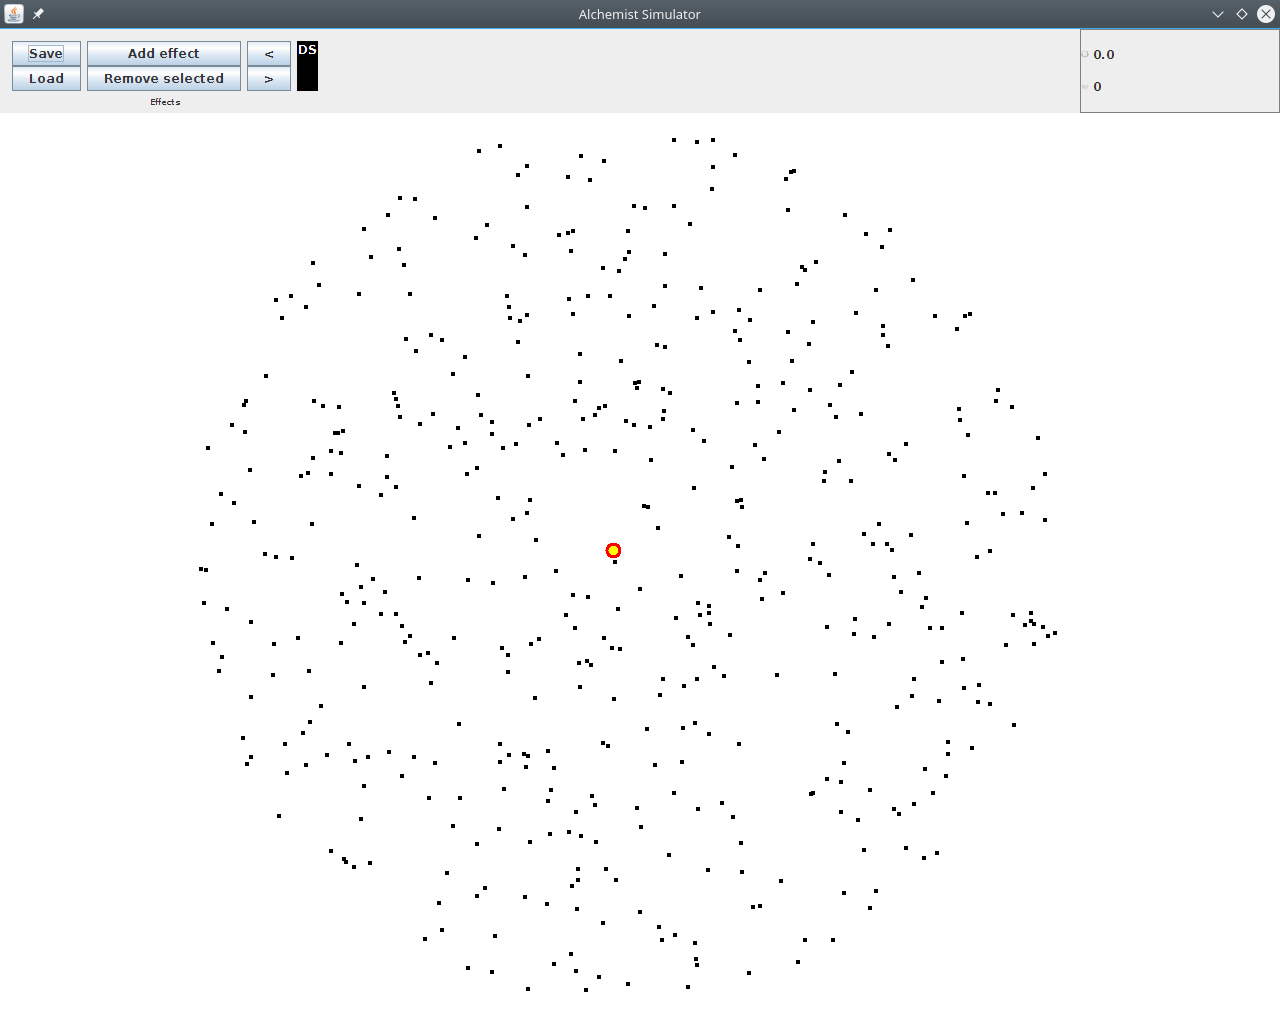
\includegraphics[scale=.29]{old/window_stopped_circle}}
            % \caption{Vista principale di una simulazione con l'interfaccia classica}
            % \label{fig:oldMain}
        % \end{figure}
    \end{frame}

    \begin{frame}
        \frametitle{\insertsection}

        
    \end{frame}

    \section*{Bibliografia}\label{sec:bib}
    \begin{frame}
        \frametitle{\insertsection}
        % per quanto non citato esplicitamente, Effective Java (2nd Edition) di Joshua Bloch ha dato il suo contributo alla scrittura del codice
        \nocite{Bloch:2008:EJ:1377533}
        \printbibliography
    \end{frame}

\end{document}
